% !TEX root = ../thesis.tex
\chapter{Methods}\label{chap:methods}

This
\published{Part of the research presented in this chapter has been published as\\ \textit{Doe J., \href{http://dx.doi.org/10.2514/1.J056710}{\mkbibquote{Some interesting journal paper,}}} AIAA Journal,  \textit{Vol. 56, No. 4, 2018, pp. 1519–1531.} }%
chapter discusses something. \lipsum[1]

\begin{figure}[ht]
   \begin{fullwidthfig}
     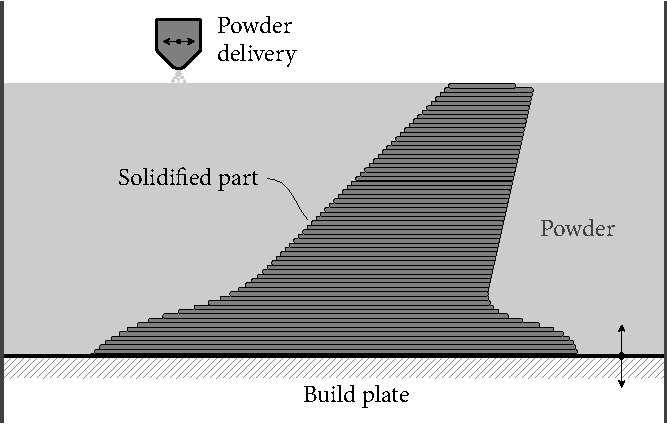
\includegraphics[width=0.9\fullwidth]{figures/example/powder_based}
   \end{fullwidthfig}
   \captionb[Shorter caption for in the LOF.]{This is some exciting figure, generated in Tikz. Note how the caption is below the figure.}{fig:tikz}
\end{figure}

 \lipsum[2]

 \begin{figure}[ht]
   \begin{sidecaption}[Some temporary figure.]{This will eventually have some exciting figure. Note how the caption is alongside the figure}[fig:temp]
     \todofig
   \end{sidecaption}
 \end{figure}

Now we are adding some citations next to the body of the text.\cite{drela1999integrated,theodorsen1935general,weissinger_naca}
\lipsum[3]
Down the line, if you cite the same article again, the number is repeated.\cite{drela1999integrated}
If you click the number in the text, you are taken to the bibliography---same for clicking the number of the sidenote.
If you click the title of the article in the margin, you are taken to article itself (through the DOI, ISBN, or website in the bibliography)---same for clicking the title in the bibliography itself.
If you click the number in ``cited on...'' in the bibliography's margin, you are taken back to the text where the article was cited.

Finally, you can also add sidenotes to the text, like so.\sidenote{Some interesting tidbit of information that was not important enough for the main text.}
Please \textit{do not} use footnotes.
